\documentclass[../main]{subfiles}
\begin{document}
\section{El problema de la Gravedad Newtoniana}\label{part2.1}
        \begin{margintable}\vspace{.8in}\footnotesize
		\begin{tabularx}{\marginparwidth}{|X}
		  Section~\ref{part2.1}. Gravedad Newtoniana\\
            Section~\ref{part2.2}. Principio de Equivalencia \\
            Section~\ref{part2.3}. Relatividad Especial\\
            Section~\ref{part2.4}. Transformaciones de Lorentz\\
            Section~\ref{part2.5}. Diagramas de Espacio-tiempo\\
            Section~\ref{part2.6}. Cinemática y dinámica relativista\\
		\end{tabularx}
	\end{margintable}
 
En mecánica clásica el potencial gravitacional de una distribución de materia $\rho(\vec{x}, t)$ viene dada por la ecuación de Poisson:
\begin{equation}
    \nabla^2 \Phi(\vec{x}, t)=-4\pi G\rho(\vec{x}, t) \ \rightarrow \ \Phi(\vec{x}, t)=-G \int \mathrm{d}^3 x' \dfrac{\rho(\vec{x}, t)}{|\vec{x}-\vec{x}'|}
\end{equation}

Sin embargo $\Phi(\vec{x}, t)$ no puede cambiar instantaneamente por cambios en la distribución de materia $\rho(\vec{x}, t)$. En electromagnetismo tenemos un problema similar:
\begin{equation}
    \nabla^2 \Phi=-\dfrac{\rho(\vec{x}, t)}{\epsilon_0} \ \rightarrow \ \Phi(\vec{x}, t)=\dfrac{1}{4\pi \epsilon_0}\int \mathrm{d}^3 x' \dfrac{\rho(\vec{x}, t)}{|\vec{x}-\vec{x}'|}
\end{equation}
\begin{adjustwidth}{0pt}{-100pt}
la solución: \textcolor{blue}{Encontrar las ecuaciones covariantes que sean consistentes con diferentes observadores.}

\textcolor{red}{Hint: Ecuaciones de Maxwell}
\begin{equation}
    \begin{aligned}
        \partial_{\mu} F^{\mu\nu}&=J^{\nu} \\
        \partial_{\mu}{}^{*} F^{\mu\nu}&=0
    \end{aligned}
    \left\{
    \begin{aligned}
        A^{\mu}&=(\phi, \vec{A})\\
        J^{\mu}&=(\rho, \vec{J})\\
        F_{\mu\nu}&=\partial_{\mu} A_{\nu}-\partial_{\nu}A_{\mu}
    \end{aligned}
    \right.
\end{equation}
Donde ${}^* F_{\mu\nu}$ es el dual de $F_{\mu\nu}$.\footnote{$*f_{\mu\nu}=\dfrac{1}{2}\epsilon_{\mu\nu}^{\lambda \theta}F_{\lambda\theta}$.} 

Estas ecuaciones son invariantes bajo transformaciones de Lorentz(y cambiando $\partial_{\mu}\rightarrow \nabla_{\mu}$ son covariantes).

\textcolor{red}{La Relatividad General plantea ecuaciones covariantes bajo difeomorfismos para la gravedad.}

\section{Principio de Equivalencia}\label{part2.2}
Existen tres formas del principio de equivalencia en Relatividad General:

\definicion{ \textcolor{red}{Principio de equivalencia débil}(Galileano)}
\begin{itemize}
    \item La masa inercial es igual a la masa gravitacional.
    \item Un campo gravitacional uniforme es indistinguible de una aceleración uniforme.
    \item Un observador en caída libre no medira ningún campo gravitacional.
\end{itemize}
\begin{center}
    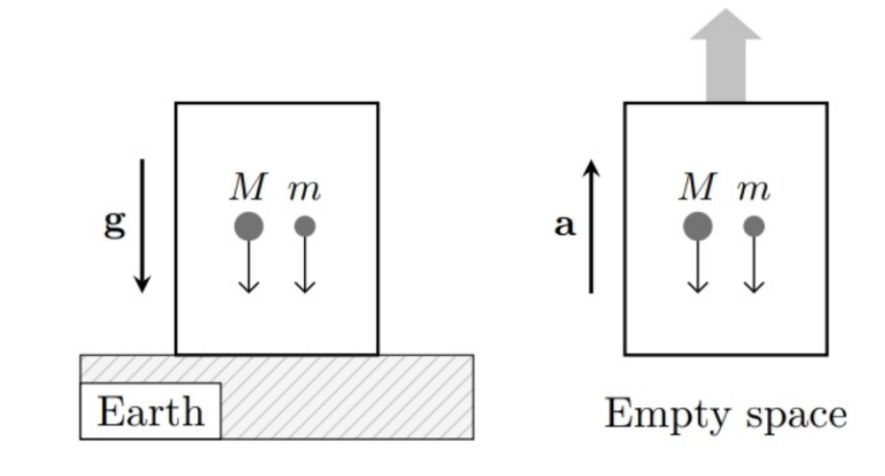
\includegraphics[scale=0.5]{img/imgRG2.1.PNG}
\end{center}

\definicion{\textcolor{red}{Principio de equivalencia de Einstein}(EEP.)}
\begin{itemize}
    \item Ningún experimento puede distinguir entre un campo gravitacional uniforme y una aceleración constante.
    \item Localmente, es posible encontrar un sistema de coordenadas inercial.
    \item En una región suficientemente pequeña las leyes de la naturaleza toman la misma forma que en un sistema de coordenadas no acelerado.
\end{itemize}
\begin{center}
    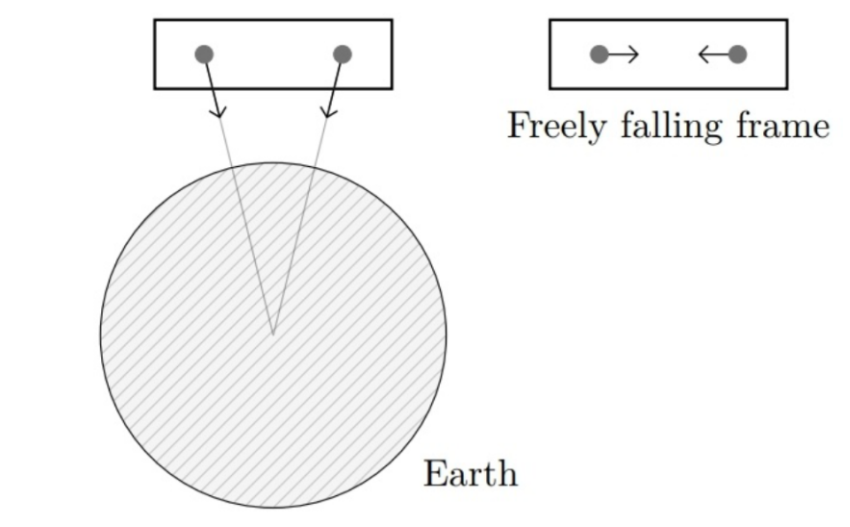
\includegraphics[scale=0.4]{img/imgRG2.2.PNG}
\end{center}

\definicion{\textcolor{red}{Principio de equivalencia fuerte}}
\begin{itemize}
    \item La dinámica interna de un sistema gravitacional no puede ser alterada por campos gravitacionales externos(Existen teorías que violan esto Brand-Dicke, HOND, etc.) más allá de las leyes de marea.
    \item Todas las leyes de la naturaleza son las mismas en un campo gravitacional uniforme y en el sistema de referencia acelerado equivalente.
    \item $G$ es una constante en el tiempo.
\end{itemize}

\section{Relatividad Especial}\label{part2.3}
\definicion{\textcolor{red}{Postulados de la Relatividad especial}}
\begin{enumerate}
    \item Las leyes de la naturaleza son las mismas en todos los sistemas inerciales.
    \item La velocidad de la luz es constante en todos los sistemas inerciales.
\end{enumerate}
Para una manifold equipada con una métrica $g_{\mu\nu}$ tenemos que las distancias $\mathrm{d}\tau$ vienen dadas por:
\begin{equation}
    \mathrm{d}\tau^2=-g_{\mu\nu}\mathrm{d}x^{\mu}\mathrm{d}x^{\nu}
\end{equation}

Como vimos anteriormente, localmente una manifold diferenciable con métrica $g_{\mu\nu}$ puede ser aproximada por:
\begin{equation}
    g_{\mu\nu} \approx \eta_{\mu\nu},
\end{equation}
para un vecindario con $\epsilon\rightarrow 0$.

Esta métrica $\eta_{\mu\nu}$(llamada de Minkowski para signatura pseudoriemanniana) permite definir el tiempo $\mathrm{d}\tau$. Usando el primer postulado para dos observadores en $x^{\mu}$ y $x^{\mu'}$ el elemento de línea $\mathrm{d}\tau^2$ viene dado por:
\begin{equation}
    \mathrm{d}\tau^2=-\mathrm{d}t^2+\mathrm{d}\vec{x}^2=-\mathrm{d}t^{'2}+\mathrm{d}\vec{x}^{'2}
\end{equation}
Las transformaciones más generales que dejan invariante $\mathrm{d}\tau$, vienen dadas por el grupo $O(1, 3)$.

\section{Transformaciones de Lorentz}\label{part2.4}
Como vimos anteriormente, en general, $\mathrm{d}\tau^2$ es invariante bajo $O(1, 3)$, \textcolor{blue}{el grupo de Lorentz}\footnote{En general el grupo de Lorentz puede ser homogeneo si solo se incluye $\Lambda^{\mu}_\nu$ al transformar $x^{\mu}$ o inhomogeneo $x^{\mu} \rightarrow x^{'\mu}=\Lambda^{\mu}_{\nu}x^{\nu}+a^{\mu}$, esto se conoce como grupo de Poincare.}, donde podemos derivar las transformaciones de Lorentz $\Lambda^{\mu}_{\nu}$. Para las coordenadas $x^{\mu}$ tenemos que:
\begin{equation}
    x^{\mu} \rightarrow x^{'\mu}=\Lambda^{\mu}_{\nu} x^{\nu}
\end{equation}

Esta transformación preserva la norma de $x^{\mu}$ en la manifold con métrica $\eta_{\mu\nu}$ con $\eta_{\mu\nu}=\operatorname{diag} (-1, 1, 1, 1)$, esto es:
\begin{equation}
    \Lambda^{\mu}_{\rho} \eta^{\rho\theta}(\Lambda^{-1})^{\nu}_{\theta}=\eta^{\mu\nu}
\end{equation}

Las transformaciones $\Lambda^{\mu}_{\rho}$ mas generales que se pueden escribir para la ecuación anterior vienen dadas por la matriz:
\begin{equation}
    \Lambda^{\mu}_{\nu}=
    \begin{pmatrix}
        \gamma & -\gamma \beta_x & -\gamma \beta_y & -\gamma\beta_z \\
        -\gamma \beta_x & 1+(\gamma-1)\hat{\beta}^2_x & (\gamma-1)\hat{\beta}_y\hat{\beta}_x & (\gamma-1)\hat{\beta}_z\hat{\beta}_x \\ 
        -\gamma \beta_y & (\gamma-1)\hat{\beta}_x\hat{\beta}_y & 1+(\gamma-1)\hat{\beta}^2_y & (\gamma-1)\hat{\beta}_z\hat{\beta}_y \\
        -\gamma \beta_z & (\gamma-1)\hat{\beta}_x\hat{\beta}_z & (\gamma-1)\hat{\beta}_y\hat{\beta}_z & 1+(\gamma-1)\hat{\beta}_z
    \end{pmatrix}
\end{equation}
donde $\hat{\beta}_i=\beta_i/\beta$, $i=(x, y, z)$.

De donde la condición $\Lambda \eta \eta^{-1}=\eta$, se tiene que 
\begin{equation}
    (\Lambda^0_0)^2=1+\sum_{i=1}^3 (\Lambda^{i}_0)^2 \geq 1
\end{equation}
y $(\det \Lambda)^2=1$, de donde se sigue que las transformaciones de Lorentz puede dividirse en cuatro componentes:

\begin{table}[H]
    \begin{adjustwidth}{0pt}{-100pt}
    \begin{center}
        \begin{tabular}{|c|c|c|c|}
            \hline
            Nombre & $\det \Lambda$ & $\Lambda^0_0$ & Notación \\ \hline
            Propia Ortocróna & $+1$ & $> 0$ & $L^{\uparrow}_{+}$ \\ \hline
            Propia Asincróna & $+1$ & $< 0$ & $L^{\uparrow}_{-}$ \\ \hline
            Impropia Ortocróna & $-1$ & $> 0$ & $L^{\downarrow}_{+}$ \\ \hline
            Impropia Asincróna & $-1$ & $< 0$ & $L^{\downarrow}_{-}$ \\ \hline
        \end{tabular}    
    \end{center}
    \end{adjustwidth}
\end{table}

Donde bajo paridad $\mathbb{P} (\vec{x}\rightarrow -\vec{x})$ e inversión temporal $(t\rightarrow -t)$ podemos mapear una transformación de Lorentz propia Ortocróna(que preserva la dirección del tiempo):
\begin{center}
    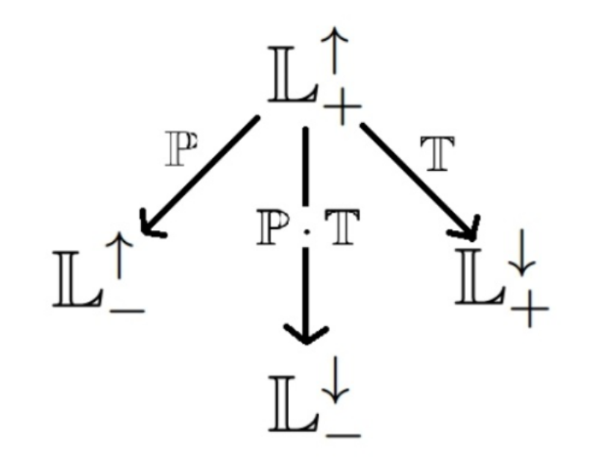
\includegraphics[scale=0.5]{img/imgRG2.3.PNG}
\end{center}

\teorema{} Toda transformación del grupo de Lorentz restringido $L^{\uparrow}_{+}$ puede escribirse como una rotación propia y un boost.

Prueba: Escribiendo $\delta \Lambda^{\mu}_{\nu}$ en función de sus generadores tenemos que
\begin{equation}
    S\Lambda^{\mu}_{\nu}=-i\dfrac{1}{2}\theta^{\alpha\beta}(M_{\alpha\beta})^{\mu}_{\nu}
\end{equation}
donde $(M_{\alpha\beta})^{\mu}_{\nu}=i(\delta^{\mu}_{\alpha}g_{\beta\nu}-\delta^{\mu}_{\beta}g_{\alpha\nu})$, tenemos que $t^{\alpha\beta}$ es un tensor antisimétrico con $6$ componentes independientes($3$ angulos de Euler + $3$ parámetros de boost). Escribiendo $M_{\mu\nu}$ en sus componentes es fácil ver que 
\begin{align*}
    M_{ij}&=\epsilon_{ijk} J_K  \ \rightarrow \  (3 \ \text{componentes})\\
    M_{0i}&=K_i \hspace{0.8cm} \rightarrow \  (3 \ \text{componentes})
\end{align*}

Si definimos $J_K=\dfrac{1}{2}\epsilon_{klm}M^{lm}$, podemos probar que usando el algebra de Lie de $SO(3, 1)$ tenemos que $J_K$ son los generadores de $SO(3)$.
\begin{equation}
    \begin{aligned}
        [M_{\mu\nu}, M_{\rho\theta}]&=ig_{\nu\rho}M_{\mu\theta}-ig_{\mu\rho}M_{\nu\theta}-ig_{\nu\theta}M_{\mu\rho}+ig_{\mu\theta}M_{\nu\rho}\\
        [J_K, J_l]&=i\epsilon_{klm} J_m,\quad k,l,m=1, 2, 3
    \end{aligned}
\end{equation}

Donde $K_i$ son los generadores de Boost\footnote{Es posible mostrar que usando generadores de Boost $K_i$ es posible obtener una rotación: $[K_l, K_m]=-i\epsilon_{lmn}J_n$.}, por lo tanto las transformaciones de Lorentz $L^{\uparrow}_{+}$ pueden escribirse como: 
\begin{equation}
    \Lambda^{\uparrow}_{+}=e^{(-i\theta_i J_i+w_i K_i)}
\end{equation}
por ejemplo un boost en la dirección $x$, nos lleva a la transformación:
\begin{equation}
    \begin{aligned}
        t'&=t\cosh w-x\sinh w\\
        x'&=-t\sinh w+x\cosh w
    \end{aligned}
\end{equation}
si $w=\tanh^{-1}(v)$ recuperamos:
\begin{equation}
    \begin{aligned}
        t'&=\gamma(t-vx)\\
        x'&=\gamma(x-vt)
    \end{aligned}
\end{equation}
con $\gamma=\dfrac{1}{\sqrt{1-v^2}}$.

Esto trae consecuencias como la dilatación del tiempo, la contracción de la longitud, etc.

\section{Diagramas de Espacio-tiempo}\label{part2.5}
Se utilizan para representar una porción del espacio de Minkowski representando puntos del espacio-tiempo con longitud negativa\textcolor{red}{(space-like)}, nula\textcolor{red}{(null)} y positiva\textcolor{red}{(time-like)}.

\definicion{\textcolor{red}{Tiempo propio}.} Mide el tiempo transcurrido por un observador que se mueve en una trayectoria recta(Minkowski) entre los eventos. Debido a que las partículas siguen trayectorias de tipo space-like se define 
\begin{equation}
    \tau=-\eta_{\mu\nu} \Delta x^{\mu}\Delta x^{\nu}
\end{equation}
\begin{center}
    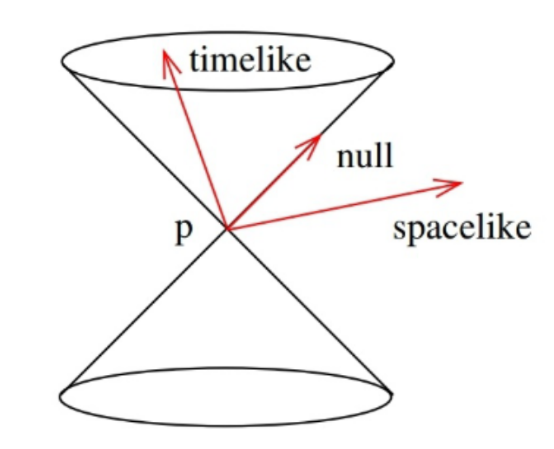
\includegraphics[scale=0.4]{img/imgRG2.4.PNG}
\end{center}

\ejemplo{Paradoja de los gemelos.} Alice, Bob en este ejemplo tenemos dos observadores en dos trayectorias diferentes, el tiempo propio que cada uno medira es distinto. 
\begin{center}
    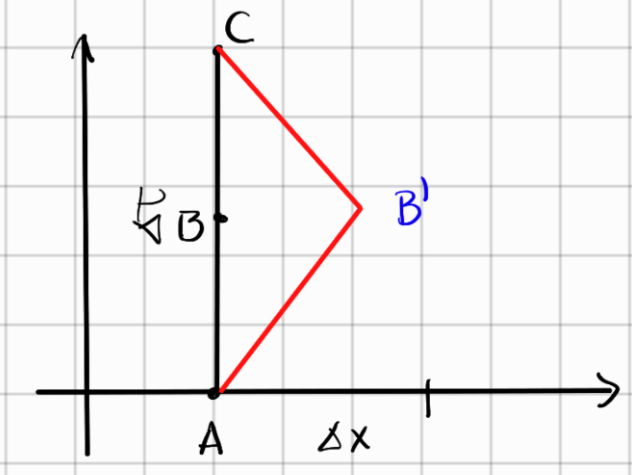
\includegraphics[scale=0.5]{img/imgRG2.5.PNG}
\end{center}
\begin{equation}
    \stackrel{\text{Bob}}{\Delta \tau_{AB'C}}=\sqrt{1-v^2}\Delta \tau < \stackrel{\text{Alice}}{\Delta \tau}
\end{equation}
Nótese que esto es posible puesto que la geometría del problema no es euclídeana.

Propiedades de los diagramas de espacio-tiempo 
\begin{enumerate}
    \item Debido al segundo postulado de la relatividad especial, ninguna trayectoria física puede ser time-like.
    \item Los diagramas de espacio-tiempo esbozan eventos que están causalmente conectados
    \item Como consecuencia de que $C$ es constante entre sistemas de referencia, los angulos relativos entre ejes de coordenadas cambian con la velocidad.
\end{enumerate}
\begin{center}
    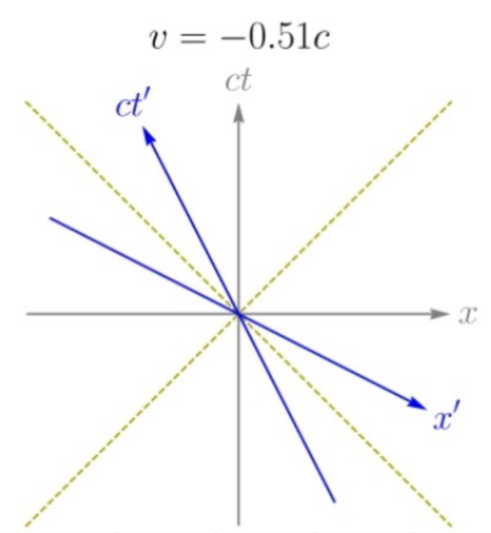
\includegraphics[width=0.3\textwidth]{img/imgRG2.6.PNG}
    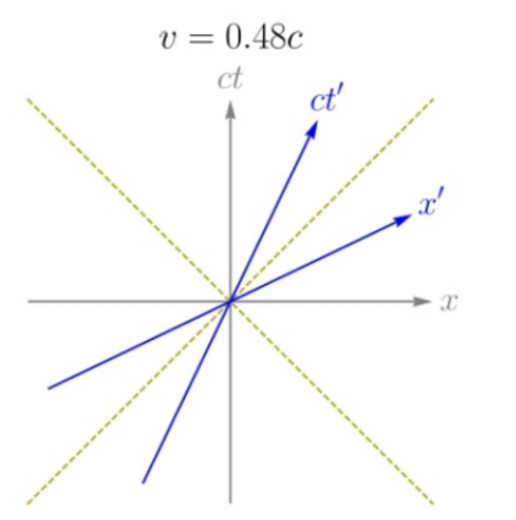
\includegraphics[width=0.3\textwidth]{img/imgRG2.7.PNG}
    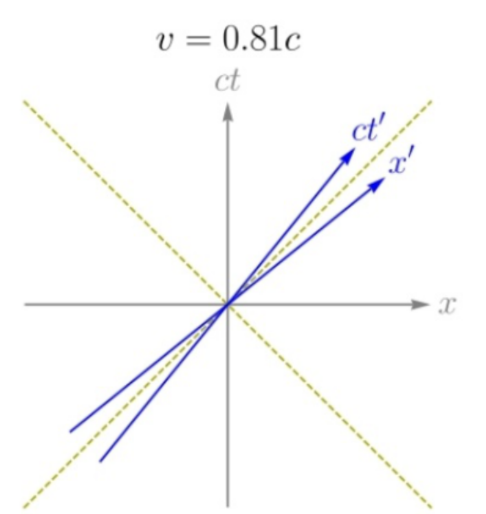
\includegraphics[width=0.3\textwidth]{img/imgRG2.8.PNG}    
\end{center}

\subsection{Cuadrivectores}
Se define como una cantidad que transforma como 
\begin{equation}
    V^{\alpha} \rightarrow V^{\alpha'}=\Lambda^{\alpha'}_{\beta} V^{\beta},\quad \alpha=1, 2, 3, 4
\end{equation}
con el sistema de coordenadas que transforma como:
\begin{equation}
    x^{\alpha}\rightarrow x^{\alpha'}=\Lambda^{\alpha'}_{\beta}x^{\beta}
\end{equation}
al vector $V^{\alpha}$ se le denomina cuadrivector contravariante para distinguirlo del cuadrivector covariante que bajo transformaciones de Lorentz viene dado por: 
\begin{equation}
    U_{\alpha} \rightarrow U_{\alpha'}=\Lambda_{\alpha'}^{\beta} U_{\beta}
\end{equation}

Donde $\Lambda_{\alpha'}^{\beta}$ es la \textcolor{red}{transformación inversa} de Lorentz tal que:
\begin{equation}
    \Lambda_{\alpha'}^{\beta} \Lambda^{\alpha'}_{\gamma}=\delta^{\beta}_{\gamma} 
    \left\{
    \begin{aligned}
        +1, & \quad \beta = \gamma \\
        0,  & \quad \beta \neq \gamma
    \end{aligned}
    \right.
\end{equation}

Se sigue que el producto de un vector contravariante con un covariante es invariante de Lorentz 
\begin{equation}
    \begin{aligned}
        U_{\alpha'}V^{\alpha'}&=\Lambda_{\alpha'}^{\beta} U_{\beta} \Lambda^{\alpha'}_{\gamma} V^{\gamma}=\left(\Lambda^{\beta}_{\alpha'} \Lambda^{\alpha'}_{\gamma}\right)U_{\beta} V^{\gamma} \\
        \left(\Lambda^{\beta}_{\alpha'} \Lambda^{\alpha'}_{\gamma}\right)U_{\beta} V^{\gamma}&=\delta^{\beta}_{\gamma} U_{\beta} V^{\gamma}=U_{\beta} V^{\beta}
    \end{aligned}
\end{equation} 

Nótese que el producto anterior puede ser escrito como 
\begin{equation}
    U_{\beta} V^{\beta}=\left(\eta_{\beta\gamma}U^{\gamma}\right)\left(\eta^{\beta\theta}V_{\beta}\right)
\end{equation}
permitiendo asignarle un vector contravariante a cada vector covariante y viceversa.
\begin{align}
    V_{\alpha}&=\eta_{\alpha\beta}V^{\beta}, \ \forall V^{\beta} \quad (\text{Index lowering}),\\
    U^{\alpha}&=\eta^{\alpha\beta}U_{\gamma}, \ \forall U_{\gamma} \quad \ (\text{Index rising})
\end{align}

Adicionalmente, el operador gradiente, bajo Lorentz, transforma usando la regla de la cadena 
\begin{equation}
    \partial_{\alpha}=\pdv{}{x^{\alpha'}}=\pdv{x^{\beta}}{x^{\alpha'}}\pdv{}{x^{\beta}}
\end{equation}

Si invertimos la transformación de $x'$ usando $\Lambda^{-1}$, esto es
\begin{equation}
    x^{\gamma}=\Lambda^{\gamma}_{\alpha} x^{\alpha}
\end{equation}
la derivada $\partial_{\alpha}$ transforma como:
\begin{equation}
    \partial_{\alpha}=\Lambda^{\beta}_{\alpha} \partial_{\beta} \quad \text{donde} \quad \partial_{\alpha}=\pdv{}{x^{\alpha}}
\end{equation}

Siguiendo estas reglas es facil ver que operadores como divergencia $\vec{\nabla}\cdot$ y D'Alambertiano $\Box$ son invariantes.

De forma analoga, un tensor transforma de forma analoga a los vectores o covectores, para un tensor de tipo $(m, n)$ transformara con $m$ transformaciones de Lorentz para cada índice y $n$ transformaciones inversas por cada dual base usado en el tensor.
\begin{equation}
    \begin{aligned}
        T^{\mu'_1 \mu'_2 \cdots \mu'_m}_{\nu'_1 \nu'_2 \cdots \nu'_n}=\overbrace{\left(\Lambda^{\mu'_1}_{\mu_1} \Lambda^{\mu'_2}_{\mu_2}\cdots \Lambda^{\mu'_m}_{\mu_m}\right)}^{m \ \text{veces}} \underbrace{\left(\Lambda^{\nu_1}_{\nu'_1}\Lambda^{\nu_2}_{\nu'_2}\cdots \Lambda^{\nu_n}_{\nu'_n}\right)}_{n \ \text{veces}} T^{\mu_1\mu_2 \cdots \mu_m}_{\nu_1\nu_2\cdots \nu_n}
    \end{aligned}
\end{equation}

Sin embargo, para un tensor como el de Levi-civita
\begin{equation}
    \epsilon^{\alpha\beta\gamma\delta}=
    \left\{
    \begin{aligned}
        +1 &\quad \text{Permutaciones pares}\\
        -1 &\quad \text{Permutaciones impares}\\
        0  &\quad \alpha=\beta=\gamma=\delta
    \end{aligned}
    \right.
\end{equation}
Se tiene que:
\begin{equation}
    \epsilon^{\alpha' \beta' \gamma' \delta'}=\dfrac{1}{\det \Lambda} \Lambda^{\alpha'}_{\alpha} \Lambda^{\beta'}_{\beta} \Lambda^{\gamma'}_{\gamma} \Lambda^{\delta'}_{\delta}\epsilon^{\alpha\beta\gamma\delta}
\end{equation}
para transformaciones propias de Lorentz $\det \Lambda=+1$.

\section{Cinemática y dinámica relativista}\label{part2.6}
\definicion{\textcolor{red}{Cuadrivelocidad:}} Se define como el vector tangente a la línea de mundo de la partícula:
\begin{equation}
    U^{\mu}=\dv{x^{\mu}}{\lambda}
\end{equation}
donde $\lambda$ parametriza la línea de mundo de la partícula, escogiendo el tiempo propio vemos que la cuadrivelocidad esta normalizada
\begin{equation}
    \mathrm{d}\tau^2=-\eta_{\mu\nu} \mathrm{d}x^{\mu}\mathrm{d}x^{\nu},\quad \eta_{\mu\nu}U^{\mu}U^{\nu}=-1
\end{equation}
nótese que para trayectorias \textcolor{red}{nulas} $\mathrm{d}\tau=0$, por lo tanto no es posible usarlo como parámetro.

\definicion{\textcolor{red}{Cuadrimomentum:}} Se define en función de $U^{\mu}$:
\begin{equation}
    P^{\mu}=mU^{\mu}
\end{equation}
las componentes de $U^{\mu}$ vienen dadas por 
\begin{equation}
    U^{\mu}=\left(\dv{t}{\tau}, \dv{\vec{x}}{\tau}\right)=(\gamma, \gamma \vec{v})
\end{equation}
luego $P^{\mu}$:
\begin{equation}
    P^{\mu}=(m\gamma, \gamma m\vec{v})
\end{equation}
vemos que la componente $P^0$ es igual a la energía de la partícula. ($c=1$)
\begin{equation}
    \begin{aligned}
        E&=m\gamma \quad \text{con} \quad \gamma=\dfrac{1}{\sqrt{1-\beta^2}} \\
        \vec{P}&=m\gamma \vec{v}
    \end{aligned}
\end{equation}
En el límite de $V\rightarrow 0$, las expresiones se reducen a las definiciones de energía y momento lineal clásicos 
\begin{equation}
    \begin{aligned}
        E&=m+\dfrac{1}{2}mv^2+\Theta(v^3) \\
        \vec{P}&=m\vec{v}+\Theta(\vec{v}^3)
    \end{aligned}
\end{equation}

\definicion{\textcolor{red}{Fuerza Relativista:}} De la definición de $P^{\mu}$ podemos encontrar la fuerza relativista:
\begin{equation}
    f^{\mu}=\dv{P^{\mu}}{\tau}=m\dv[2]{x^{\mu}}{\tau}
\end{equation}

\ejemplo{} La fuerza de Lorentz en electromagnetismo
\begin{equation}
    f^{\mu}=qU^{\lambda} F^{\mu}_{\lambda}
\end{equation}


\section*{Problemas 2}
\begin{enumerate}
    \item \textbf{Derivada de Lie}
    \begin{enumerate}
        \item Utiliza la regla de Leibniz para derivar la fórmula para la derivada de Lie de una 1-forma $\omega$, válida en cualquier base de coordenadas:
        \begin{equation}
            (\mathcal{L}_X \omega)_{\mu}=X^{\nu} \partial_{\nu} \omega_{\mu}+\omega_{\nu} \partial_{\mu} X^{\nu}.
        \end{equation}
        Sugerencia: Considera $(\mathcal{L}_X \omega)(Y)$ para un campo vectorial $Y$.
        \item Muestra que la derivada de Lie de un tensor $(0, 2)$, $g$ es:
        \begin{equation}
            (\mathcal{L}_X g)_{\mu\nu}=X^{\rho} \partial_{\rho} g_{\mu\nu}+g_{\mu\rho}\partial_{\nu}X^{\rho}+g_{\rho\nu}\partial_{\mu}X^{\rho}.
        \end{equation}
    \end{enumerate}
    \item \textbf{Formas} 
    \begin{enumerate}
        \item Sea $\omega$ una p-forma y $\eta$ una q-forma. Demuestra que la derivada exterior satisface las propiedades 
        \begin{itemize}
            \item $\mathrm{d}(\mathrm{d} \omega)=0$.
            \item $\mathrm{d}(\omega \wedge \eta)=(\mathrm{d} \omega)\wedge \eta+(-1)^p \omega \wedge \mathrm{d}\eta$.
            \item $\mathrm{d}(\varphi^* \omega)=\varphi^*(\mathrm{d}\omega)$ donde $\varphi: M \rightarrow N$ para manifolds $M$ y $N$.
        \end{itemize}
    \end{enumerate}
    \item \textbf{Transformaciones de Coordenadas Infinitesimales}\\
    Un campo vectorial se puede ver como una transformación de coordenadas infinitesimal. Considera la familia de transformaciones de coordenadas 
    \begin{equation}
        x^{\mu} \rightarrow y^{\mu}=y^{\mu}(x^{\mu}, \sigma)
    \end{equation} 
    donde $\sigma$ es un parámetro continuo que controlará cuán infinitesimal es la transformación. Tomaremos $y^{\mu}(x^{\mu}, \sigma=0)=x^{\mu}$, y definimos 
    \begin{equation}
        v^{\mu} \equiv \pdv{y^{\mu}}{\sigma}
    \end{equation}

    En el límite de $\sigma$ pequeño, entonces tenemos 
    \begin{equation}
        y^{\mu}=x^{\mu}+\sigma v^{\mu}+\cdots 
    \end{equation}
    y decimos que el vector $v^{\mu}$ genera esta transformación infinitesimal de coordenadas. 
    \begin{enumerate}
        \item Demuestra que $v^{\mu}$ se transforma como un vector.
        \item Considera el espacio plano tridimensional en coordenadas cartesianas $x^{i}$, $i=1, 2, 3$. Muestra que los vectores 
        \begin{equation}
            R=\partial_1, \ T=\partial_2, \ S=\partial_3
        \end{equation}
        generan traslaciones infinitesimales en las direcciones $x^1, x^2$ y $x^3$, respectivamente. Sugerencia: La respuesta aquí es directa.
        \item En el espacio tridimensional, considera los tres vectores 
        \begin{equation}
            v=x^3\partial_3-x^3\partial_2, \ \omega=x^3\partial_1-x^1\partial_3, \ q=x^1\partial_2-x^2\partial_1
        \end{equation}

        Muestra que estos vectores generan rotaciones infinitesimales alrededor de los ejes $x^1, x^2$ y $x^3$, respectivamente. Sugerencia: Escribe primero una rotación a lo largo de un eje, digamos $x^1$, por un ángulo $\alpha$. Luego expande esta expresión para ángulos pequeños: esto define una rotación infinitesimal.
    \end{enumerate}
    \item \textbf{Diagramas de Espacio-Tiempo}\\
    Considera un espacio-tiempo bidimensional(temporal+espacial) con $c=1$, la velocidad de la luz.
    \begin{enumerate}
        \item Dibuje un diagrama de espacio-tiempo $(x, t)$, presente y dé una brave explicación de los siguientes objetos
        \begin{itemize}
            \item Un evento.
            \item Un rayo de luz.
            \item La línea de mundo de un objeto que viaja con velocidad $v<1$.
            \item La línea de mundo de un objeto que viaja con velocidad $v>1$.
            \item La línea de tiempo de un objeto acelerado.
        \end{itemize}
        \item Dibuje un diagrama de espacio-tiempo $(x, t)$ de un observador $\mathcal{O}$ en reposo. En este diagrama de espacio-tiempo, dibuje la línea de mundo de un observador $\mathcal{O}'$ que viaja con velocidad $v$ medida en el sistema de referencia en reposo de $\mathcal{O}$. ¿Cuáles son los ejes de coordenadas del diagrama de espacio-tiempo de $\mathcal{O}'$?\\
        Sugerencia: ¿Cual es su eje de tiempo? ¿Cómo se construye entonces el eje espacial?
        \item La paradoja de los gemelos es un problema clásico en la teoria de la relatividad especial que ilustra como el tiempo se dilata para un observador en movimiento respecto a otro en reposo. Imagina dos gemelos, Alice y Bob. Alice se embarca en un viaje espacial, mientras que Bob se queda en la Tierra. El viaje de Alice la lleva a una estrella a 4 años luz de distancia de la Tierra a una velocidad constante de $0.8c$, donde $c$ es la velocidad de la luz. Después de llegar a la estrella, Alice regresa inmediatamente a la tierra a la misma velocidad.
        \item Dibuja un diagrama espacio-tiempo para ilustrar el viaje de Alice y Bob en el marco de referencia de Bob(la tierra) y un diagrama para ilustrar el viaje de Alice y Bob en el marco de referencia de Alice(la nave espacial). Marca los eventos clave en el diagrama, como la partida y llegada de Alice, y los puntos de inflexión en la línea de universo de Alice. Explica cómo el diagrama de Alice ayuda a resolver la aparente paradoja.
        \item Utiliza la transformación de Lorentz para calcular el tiempo que experimenta Alice durante su viaje de ida y vuelta a la estrella, y calcula el tiempo que experimenta Bob durante el viaje completo de Alice, desde su partida hasta su regreso.
    \end{enumerate}
    \item \textbf{El Grupo de Lorentz}\\
    Considera el espacio de Minkowski $\mathbb{R}^{1, 3}$ de cuatro dimensiones $\mathbb{R}^4$ equipado con la métrica de Minkowski $\eta$. Esta es una forma bilineal simétrica no degenerada $\eta: \mathbb{R}^4 \times \mathbb{R}^4 \rightarrow \mathbb{R}$ definida por 
    \begin{equation}
        \eta(e_{\mu}, e_{\nu})\equiv \eta_{\mu\nu}=
        \left\{
        \begin{aligned}
            -1 &\quad \text{para} \ \mu=\nu=0\\
            +1 &\quad \text{para} \ \mu=\nu=1, 2, 3
        \end{aligned}
        \right.
    \end{equation}
    para la base ortonormal estándar $\{e_0, e_1, e_2, e_3\}$ en $\mathbb{R}^4$. Linealidad implica que 
    \begin{equation}
        \eta(x, y)=x^T\cdot \eta \cdot y \quad \text{para} \ x,y \in \mathbb{R}^{1, 3}
    \end{equation}
    donde $\eta$ es una matriz con entradas $\eta_{\mu\nu}$. Para $x, y \in \mathbb{R}^{1, 3}$ escribimos $x\cdot y=\eta(x, y)$ y $x^2=x\cdot x$. En relatividad especial, las transformaciones de Lorentz, $\Lambda$, que relacionan dos marcos inerciales preservan la distancia en el espacio-tiempo:
    \begin{equation}
        (x-y)^2=(\Lambda(x-y))^2 \ \text{para todos} \ x, y \in \mathbb{R}^{1, 3}.
        \label{ecproblema}
    \end{equation} 
    Esto lleva ala definicion del grupo de Lorentz 
    \begin{equation}
        O(1, 3)=\{\Lambda \in GL(4, \mathbb{R})| \Lambda^T\eta \Lambda=\eta \}
    \end{equation}
    \begin{enumerate}
        \item Muestre que $\Lambda \in O(1,3)$ efectivamente cumple la ecuación \eqref{ecproblema}.
        \item Muestre que $O(1, 3)$ efectivamente es un grupo.
        \item Muestre que $\Lambda^T \eta \Lambda=\eta$ escrita en componentes se lee $\eta_{\rho\sigma}\Lambda^{\rho}_{\mu}\Lambda^{\sigma}_{\nu}=\eta_{\mu\nu}$.
        \item Muestre que $|\Lambda^0_0|\geq 1$ y que $|\det \Lambda|=1$. Con esto argumente que el grupo de Lorentz consta de cuatro ramas(que no están conectadas de forma continua entre sí.) Sugerencia: Usa $\det (1+\epsilon\lambda)=1+\epsilon \tr \lambda+\mathcal{O}(\epsilon^2)$.
        \item Muestre que el subconjunto $SO^+(1, 3)=\{\Lambda \in O(1, 3)| \det \Lambda =1, \Lambda^0_0\geq 1\}$ forma un subgrupo de $O(1, 3)$ llamado el grupo de Lorentz ortocrono propio.
    \end{enumerate}
\end{enumerate}
\end{adjustwidth}
\end{document}